\documentclass{article}
\usepackage{graphicx} % Required for inserting images

\title{Bilgisayarla Görme Projesi Raporu \\ \large Proje Konusu: Image Captioning \\ Dersin Yürütücüsü: Oğuz Altun}
\author{Muhammed Kayra Bulut-23501059}
\date{Kasım 2023}
\usepackage{multirow}
\begin{document}
\maketitle

\section{Giriş}

\subsection{Projenin Amacı}
Bu projenin temel amacı, derin öğrenme ve bilgisayarla görme tekniklerini kullanarak otomatik görüntü alt yazılandırma sistemi geliştirmektir. Sistem, verilen bir görüntüyü analiz edecek ve içeriğini açıklayan kısa ve anlamlı bir metin üretecektir. Bu teknolojinin potansiyel uygulama alanları arasında görsel içeriklerin aranabilirliğinin artırılması, görsel engelliler için erişilebilirlik çözümleri ve otomatik içerik üretimi bulunmaktadır.
\subsection{Görüntü İşleme (Image Processing) Nedir?}
Görüntü işleme, dijital görüntüler üzerinde çeşitli işlemler yaparak bu görüntüleri iyileştirmek, analiz etmek ve bazı sonuçlar çıkarmak için kullanılan bir bilgisayar bilimi dalıdır. Bu alandaki temel işlemler arasında görüntü geliştirme ve restorasyon, gürültünün azaltılması, kenar tespiti ve görüntü sınıflandırma yer alır \cite{stefanini2022show}. Görüntü işleme, çeşitli alanlarda, özellikle tıbbi görüntüleme, uydu görüntüleme, robotik ve güvenlik sistemlerinde geniş bir uygulama yelpazesi sunar \cite{sharma2020image}. Bilgisayarla görme (computer vision), görüntü işlemenin ötesine geçerek, görüntülerdeki nesneleri, sahneleri ve etkinlikleri anlamaya ve yorumlamaya odaklanır. Görüntü işlemenin en ilgi çekici uygulamalarından biri, otomatik görüntü alt yazma (image captioning) olup, bu alanda yapılan çalışmalar, derin öğrenme tekniklerinin kullanılmasını içerir \cite{vinyals2016show} \cite{aneja2018convolutional}.

\subsection{Doğal Dil İşleme (NLP) Nedir?}
Doğal Dil İşleme (NLP), insan diliyle etkileşimde bulunabilen bilgisayar sistemlerinin geliştirilmesiyle ilgilenen bir yapay zeka ve dilbilim dalıdır. NLP'nin temel amacı, insan dilinin karmaşık yapısını anlayarak ve işleyerek bu dili kullanışlı bilgilere dönüştürmektir. Temel NLP uygulamaları arasında metin sınıflandırma, duygu analizi, dil modelleme, otomatik özet çıkarma ve dil çevirisi bulunur \cite{hossain2019comprehensive}. Görüntü alt yazılandırmada NLP, üretilen görsel özellikleri anlamlı ve doğal görünen metin ifadelerine dönüştürmek için hayati bir rol oynar \cite{vinyals2016show} \cite{yao2017boosting}. Bu süreç, derin öğrenme tekniklerinin ve dikkat mekanizmalarının kullanılmasıyla desteklenir \cite{you2016image} \cite{cornia2020meshed}.

\subsection{Görüntü Alt Yazılandırma (Image Captioning) Nedir?}
Görüntü alt yazılandırma, bir görüntüyü tanımlayan ve açıklayan metin ifadeleri otomatik olarak üreten bir bilgisayarla görme ve doğal dil işleme görevidir \cite{aneja2018convolutional}. Bu süreç, genellikle bir "encoder-decoder" modeli kullanılarak gerçekleştirilir \cite{vinyals2016show}. Encoder, görüntüden önemli özellikleri çıkarmak için derin sinir ağlarından faydalanırken \cite{cornia2020meshed}, decoder bu özellikleri alıp anlamlı bir cümle veya ifadeye dönüştürür \cite{pan2004automatic}. Bu alanın zorlukları arasında, görüntülerdeki çeşitliliği ve karmaşıklığı doğru bir şekilde metne dökme \cite{feng2019unsupervised} ve görüntüler arasındaki ince detayları yakalayıp yorumlama yeteneği bulunur \cite{stefanini2022show}.

\newpage
\section{Proje Tasarımı ve Geliştirme}

\subsection{Veri Seti ve Ön İşleme}

Projemizde kullanılan "Flickr 8k Dataset", yapay zeka ve görüntü işleme alanlarında kritik bir öneme sahiptir. Bu özel veri seti, 8,000 adet çeşitlilik gösteren görüntülerle zenginleştirilmiş olup, her bir görüntüyü beş farklı açıdan açıklayan altyazılarla eşleştirmektedir. Bu şekilde veri kümesi yaklaşık 40.000 adet altyazı içermektedir. Bu özellik, makine öğrenimi modellerinin daha detaylı ve çeşitli veri üzerinde eğitilmesine olanak tanıyarak, algoritmaların gerçek dünya senaryolarına daha iyi adapte olmasını sağlar.

Tablo \ref{tablo:veri-seti-ornek}'de sunulan örnekler, veri setinin zenginliğini ve çeşitliliğini göstermektedir. Burada, her görüntü için farklı ifadelerle yazılmış beş adet metin içeriği bulunmakta, bu da her bir görüntüyü çok yönlü olarak anlamlandırma imkanı tanımaktadır. Özellikle, bu metinlerin manuel olarak hazırlanması, doğal dil işleme (NLP) sistemlerinin geliştirilmesi için oldukça değerli bir kaynak oluşturmaktadır.

Bu veri setinin seçimi, algoritmaların gerçek dünya koşullarında daha doğru ve etkili sonuçlar vermesine yardımcı olacak şekilde yapılmıştır. Görüntüler, tanınmış kişileri veya yerleri içermemek üzere altı farklı Flickr grubundan titizlikle seçilmiştir. Bu, etik ve gizlilik standartlarının korunmasında önemli bir adımdır ve aynı zamanda veri setinin genel kullanılabilirliğini artırmaktadır. 

\begin{table}[ht]
\centering
\caption{Örnek Veri Tablosu}
\vspace{10pt}
\begin{tabular}{|c|p{10cm}|}
\hline
\textbf{Resim Dosyası} & \textbf{Metin İçeriği} \\
\hline
\multirow{5}{*}{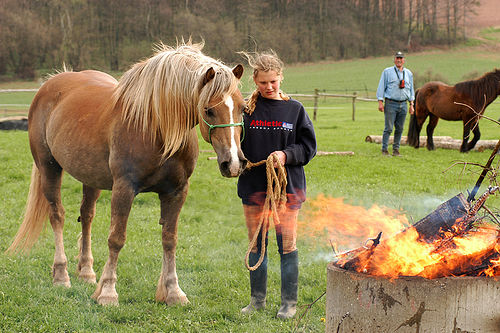
\includegraphics[width=2cm,height=2cm]{10815824_2997e03d76.jpg}} & A blonde horse and a blonde girl in a black sweatshirt are staring at a fire in a barrel. \\
& A girl and her horse stand by a fire. \\
& A girl holding a horse's lead behind a fire. \\
& "A man, and girl and two horses are near a contained fire." \\
& Two people and two horses watching a fire. \\
\hline
\multirow{5}{*}{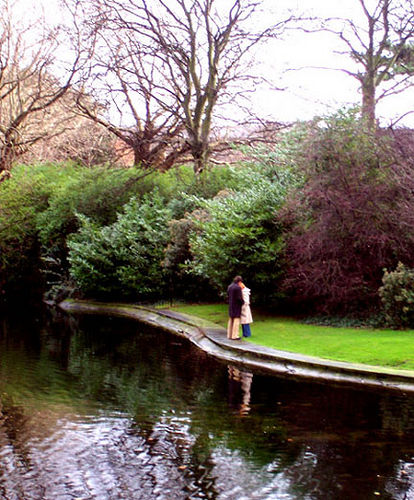
\includegraphics[width=2cm,height=2cm]{3637013_c675de7705.jpg}} & A couple stands close at the water's edge. \\
& The two people stand by a body of water and in front of bushes in fall. \\
& Two people hold each other near a pond. \\
& Two people stand by the water. \\
& Two people stand together on the edge of the water on the grass. \\
\hline
\end{tabular}
\label{tablo:veri-seti-ornek}
\end{table}

Veri setindeki görüntülerin ön işlemesi için özel bir işlev zinciri kullanılmıştır. Her bir görüntü, TensorFlow kütüphanesi kullanılarak okunmuş, JPEG formatında çözülmüş ve [310x310] piksel boyutlarına yeniden boyutlandırılmıştır. Ardından, görüntülerin renk değerleri normalize edilerek 0 ile 1 arasında bir aralığa dönüştürülmüştür.

Altyazılar için uygulanan ön işleme süreci, metinleri küçük harfe çevirme, noktalama işaretlerini ve fazladan boşlukları kaldırma adımlarını içerir. Her bir altyazı, başına '[start]' ve sonuna '[end]' tokenleri eklenerek standart bir formata dönüştürülmüştür. Bu işlemler, altyazıların model tarafından daha etkili bir şekilde işlenmesini sağlamaktadır.



\subsection{Model Mimarisi}

\subsubsection{Encoder: Görüntü Öznitelikleri Nasıl Çıkarılır}
Projenin Encoder kısmı, InceptionV3 modelini temel alır. Bu model, ImageNet ağırlıkları ile önceden eğitilmiş ve en üst katman dahil edilmeden kullanılmıştır. Modelin eğitilebilirliği kapalı tutularak, görsel içerikten öznitelik vektörleri çıkarmak için kullanılır. InceptionV3'ün çıktısı, global ortalama havuzlama (pooling) ile işlenerek yoğun bir vektör haline getirilir ve bu vektör Decoder'a iletilmek üzere hazırlanır.

\subsubsection{Transformer Encoder Katmanı}
Projede yer alan Transformer Encoder katmanı, çoklu başlık dikkat mekanizması ve yoğun katmanlardan oluşur. Bu katman, katman normalizasyonları ve derinlemesine dikkat mekanizması aracılığıyla girdi verilerini işler. Transformer Encoder, modele karmaşık dikkat ilişkilerini modellemesini sağlayarak, görsel öğeler arasındaki bağlantıları daha etkili bir şekilde anlamasına yardımcı olur.

\subsubsection{Decoder: Metin Oluşturma ve Alt Yazılandırma}
Decoder kısmı, metin ve pozisyon gömme katmanları ile birlikte çoklu başlık dikkat mekanizmaları ve yoğun katmanları içeren bir Transformer Decoder katmanından oluşur. Kendi kendine dikkat mekanizması ve Encoder-Decoder dikkat mekanizması, girdi metni ve Encoder çıktısını birleştirerek, tahmini metin çıktılarını üretir. Bu süreç, metni çözümleme ve tahmin etme kapasitesini artırarak, görüntü için uygun ve anlamlı altyazıları üretir.
\subsubsection{Transformer Modellerin Rolü}
Transformer modeller, projede, görsel ve metinsel veriler arasındaki karmaşık ilişkileri öğrenmek ve anlamlandırmak için kritik bir rol oynar. Bu modeller, çoklu başlık dikkat mekanizmalarını kullanarak, modelin hem görsel içeriğin derinlemesine analizini yapmasını hem de bu içeriğe uygun metin üretimini gerçekleştirmesini sağlar. Transformer modeller, paralel işleme yetenekleri ve uzun mesafeli bağımlılıkları etkili bir şekilde yakalama kabiliyetleri sayesinde, görsel alt yazılandırma görevinde yüksek başarı gösterir. Bu yaklaşım, modelin görsel öğeler arasındaki incelikli ilişkileri ve bunların dil ile olan bağlantılarını daha iyi anlamasına imkan tanır.


\subsubsection{Modelin Eğitim ve Test Süreçleri}
Model, eğitim ve test adımlarında kayıp ve doğruluk metriklerini hesaplar. Eğitim süreci, görsel ve metin verileri üzerinden modeli güncelleyerek, tahmin edilen altyazıların doğruluğunu ve kalitesini artırmaya yöneliktir. Test süreci ise, modelin genel performansını ve altyazı üretme yeteneğini değerlendirir.

Bu model mimarisi, görüntü ve metin verileri arasındaki karmaşık ilişkileri öğrenmek ve anlamlandırmak için gelişmiş yapay zeka tekniklerini kullanır. Encoder ve Decoder bileşenleri arasındaki etkileşim, modelin veri setindeki görüntüleri ve ilgili altyazıları etkili bir şekilde işlemesini sağlar.
\subsection{Performans Metrikleri ve Değerlendirme}
Modelin performansı, çeşitli metrikler kullanılarak değerlendirilmiştir. Bu metrikler arasında doğruluk, kayıp oranı ve belki de daha önemlisi, üretilen altyazıların kalitesini ölçen BLEU skoru gibi dil modelleme metrikleri bulunur. Eğitim sürecinde, modelin kaybı ve doğruluğu sürekli olarak izlenmiş ve optimize edilmiştir. Test aşamasında, modelin gerçek dünya verileri üzerindeki performansı, seçilen metriklerle detaylı bir şekilde analiz edilmiştir. Bu değerlendirme, modelin güçlü yönlerini ve geliştirilmesi gereken alanları ortaya koyarak, gelecekteki iyileştirmeler için yön gösterici olmuştur.



\section{Sonuçlar}

\subsection{Modelin Performans Analizi}
Modelin eğitimi 20 epoch boyunca gerçekleştirilmiştir. İlk epoch sonunda, modelin eğitim kaybı 5.4380 ve doğruluk oranı \%20.67 olarak kaydedilmiştir. İlerleyen epoch'larla birlikte modelin performansında belirgin bir iyileşme gözlemlenmiştir. Özellikle, 20. epoch sonunda modelin eğitim kaybı 2.5666'ya düşmüş ve doğruluk oranı \%44.58'e yükselmiştir. Doğrulama (validation) kaybı ve doğruluk oranları da benzer bir iyileşme eğilimi göstermiş, 20. epoch sonunda sırasıyla 3.0596 ve \%40.21 olarak kaydedilmiştir. Bu sonuçlar, modelin eğitim sürecinde sürekli olarak geliştiğini ve veri seti üzerindeki genel performansının arttığını göstermektedir.

Tablo \ref{tablo:ornek-veri-tablosu}'ye bakıldığında eğitim verilerinin bağlamından pek ayrılınmadığında modelin başarılı sonuçlar ürettiği gözükmektedir. Örneğin model kardaki çocuklar ve köpeklerin olduğu fotoğraf için "a group of children are playing in a snow" altyazısının üretmiştir. Bu üretilen çıktı fotoğrafa bakıldığında akla gelen ilk cümlelerden biridir. Ya da model yine kamp ateşi olan fotoğraf için "a group of people are sitting in a campfire at night" altyazısını üretmiştir. Bu üretilen çıktı incelendiğinde yine benzer şekilde fotoğrafa bakıldığında akla ilk gelecek cümlelerden birini model başarılı şekilde üretmiştir.

\begin{table}[!h]
\centering
\caption{Örnek Veri Tablosu}
\vspace{10pt}
\begin{tabular}{|c|p{10cm}|}
\hline
\textbf{Resim Dosyası} & \textbf{Modelin Tahmini} \\
\hline
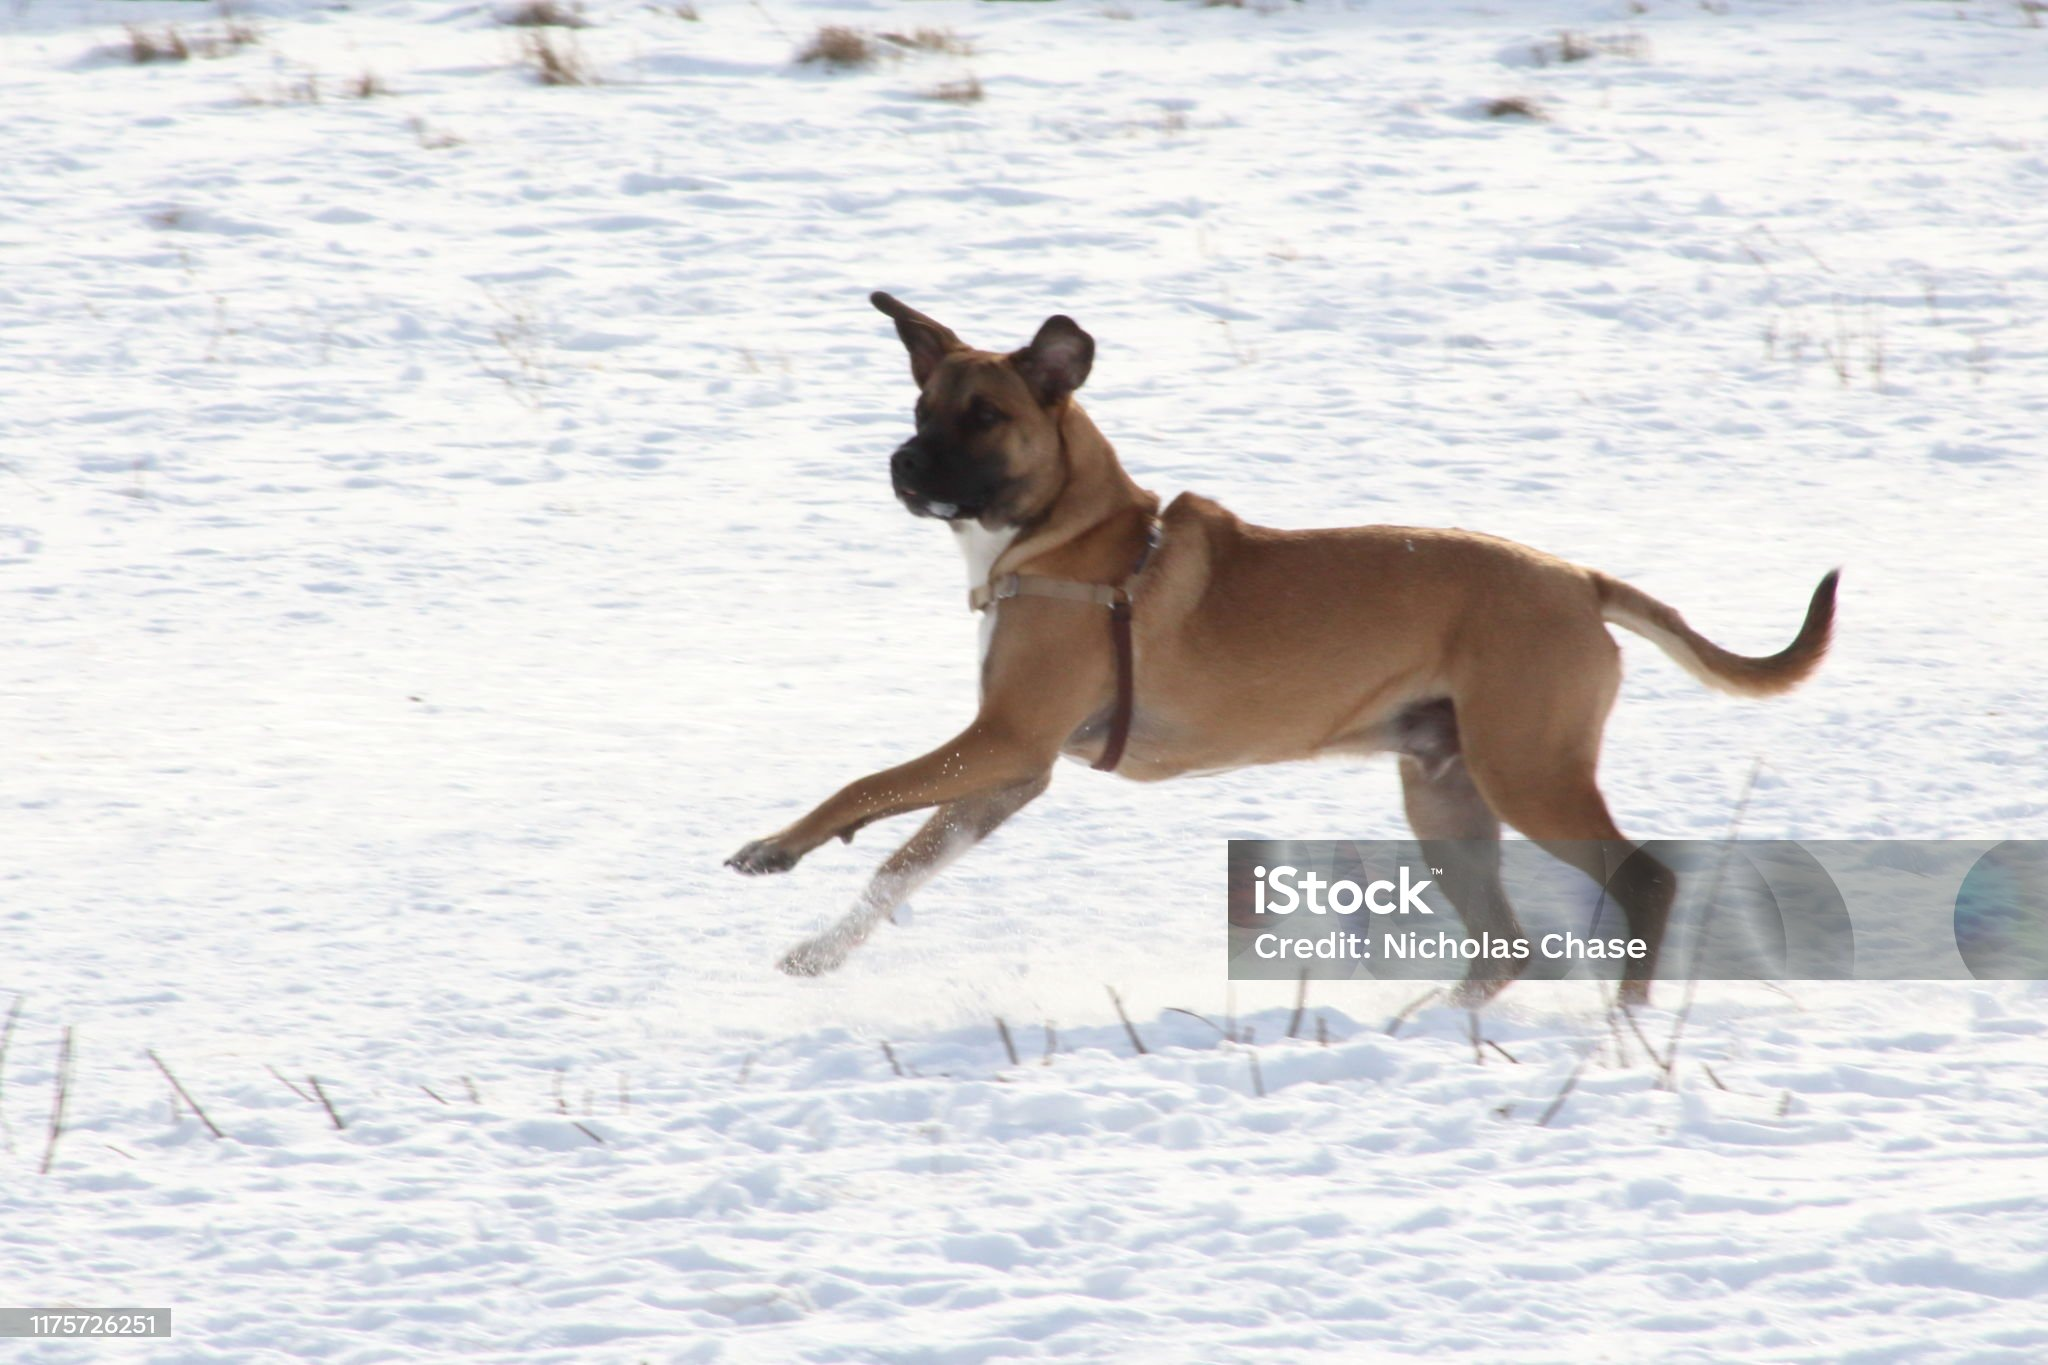
\includegraphics[width=2cm,height=2cm]{resim1.jpg} & a brown dog is running through the snow \\
\hline
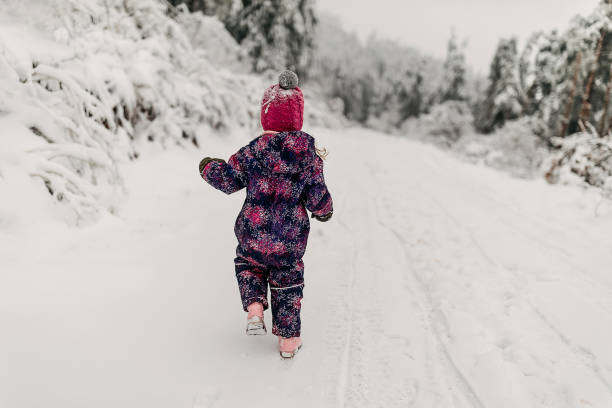
\includegraphics[width=2cm,height=2cm]{resim2.jpg} & a child in a red jacket is standing in the snow \\
\hline
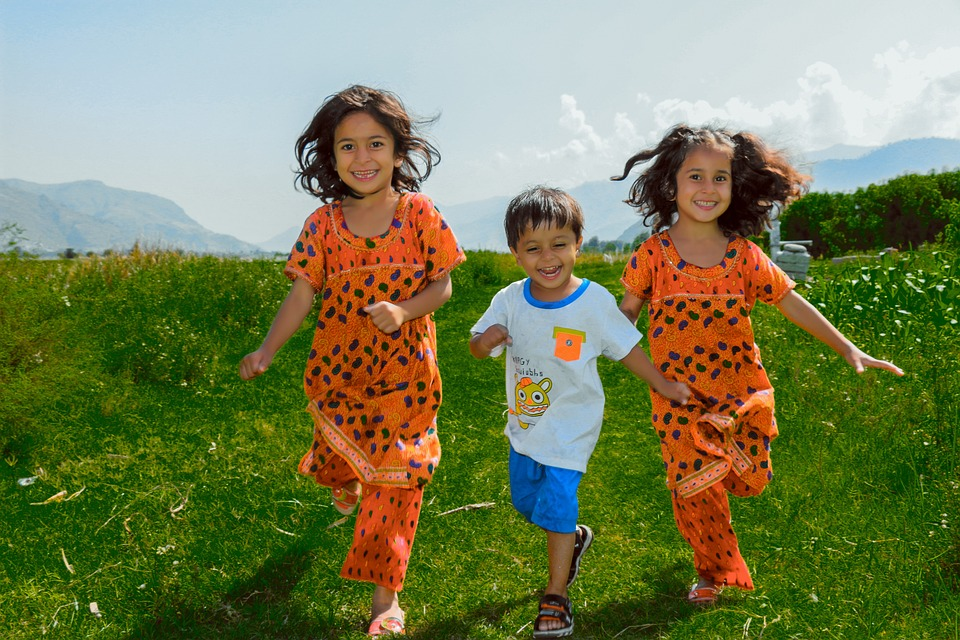
\includegraphics[width=2cm,height=2cm]{yesillikte_kosan_cocuklar.jpg} & a girl in a pink dress is standing on a sidewalk \\
\hline
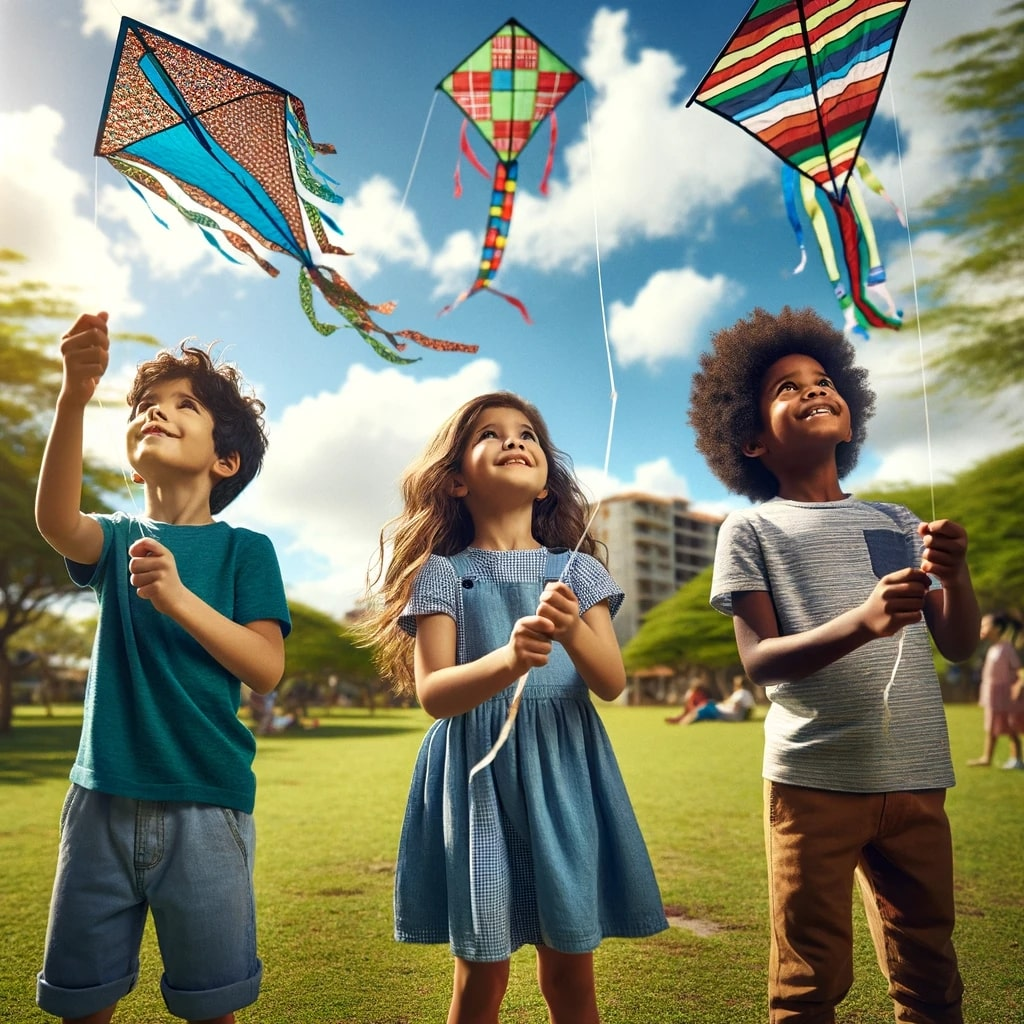
\includegraphics[width=2cm,height=2cm]{ucurtma_ucuran_cocuklar.jpg} & a group of young girls are standing in front of a crowd \\
\hline
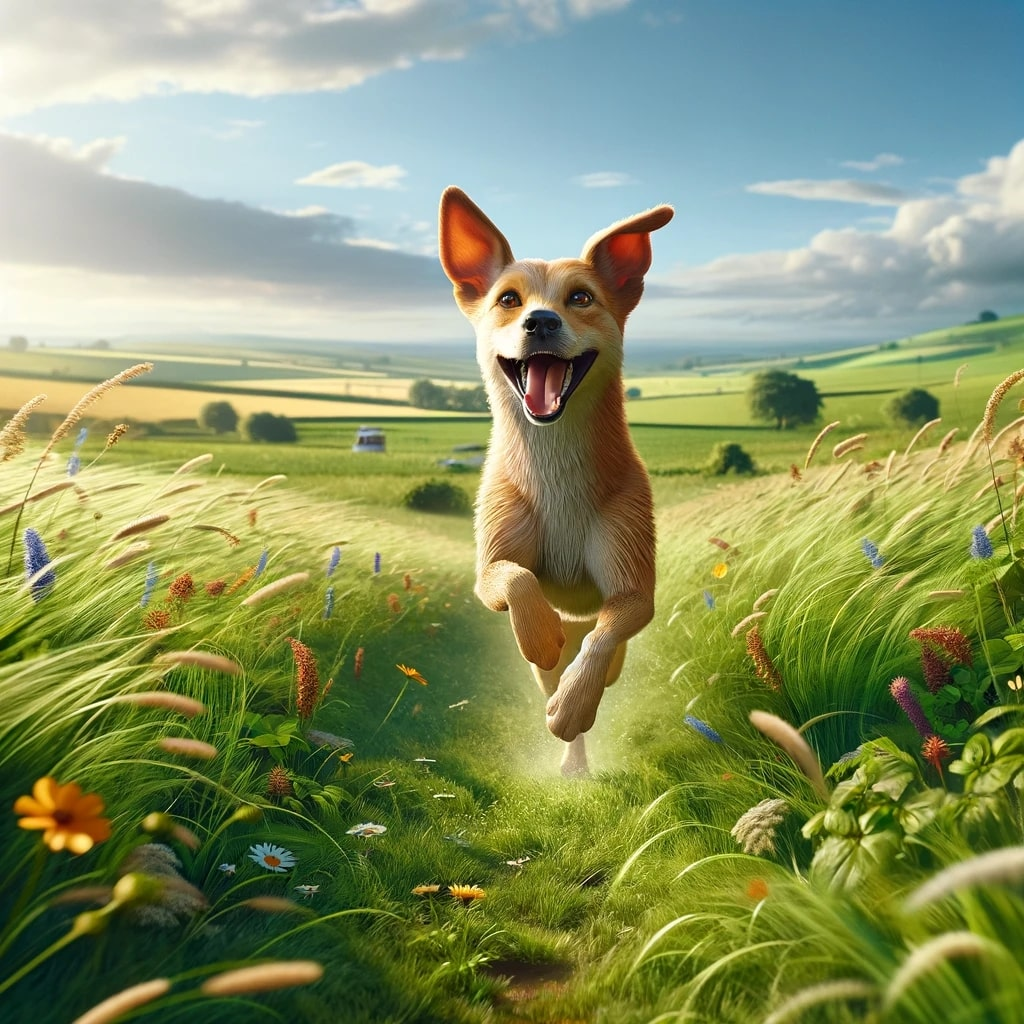
\includegraphics[width=2cm,height=2cm]{kirda_kosan_kopek_2.jpg} & a small dog is jumping in the air to catch a frisbee \\
\hline
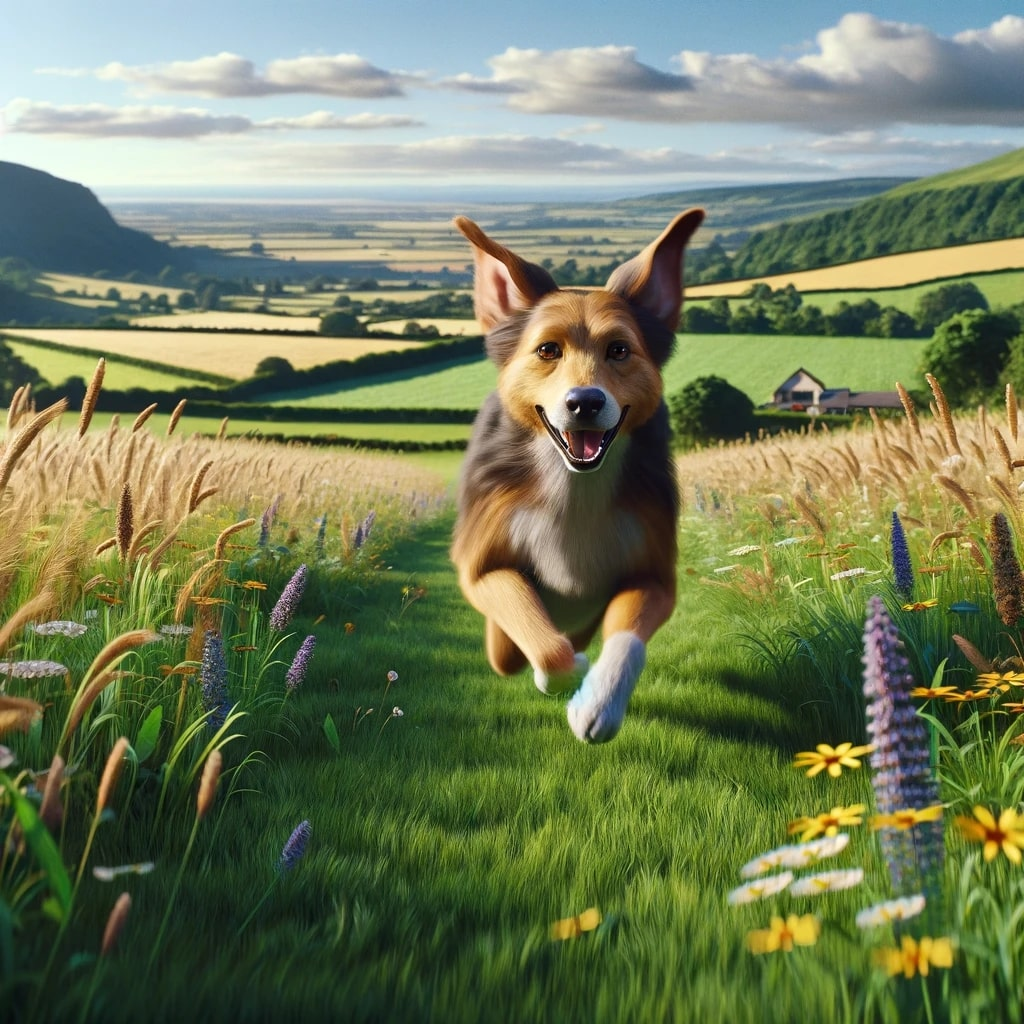
\includegraphics[width=2cm,height=2cm]{kirda_kosan_kopek_1.jpg} & a small dog runs through the grass \\
\hline
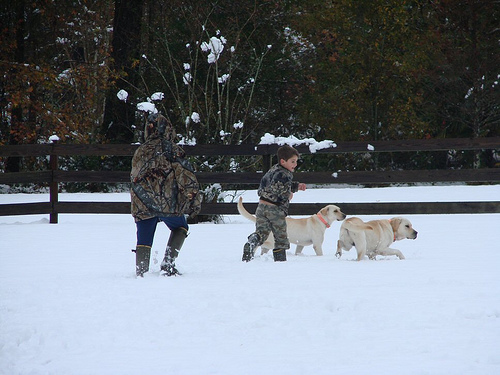
\includegraphics[width=2cm,height=2cm]{karda_yuruyen_kopekler_ve_cocuklar.jpg} & a group of children are playing in a snow \\
\hline
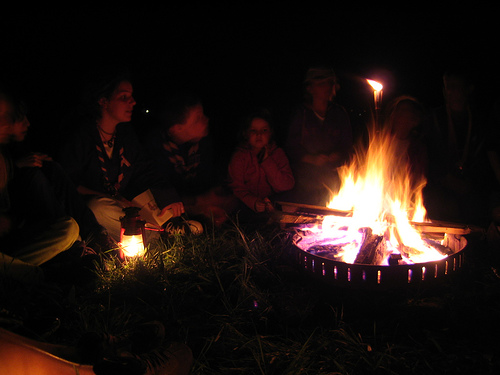
\includegraphics[width=2cm,height=2cm]{ates_etrafinda_insanlar.jpg} & a group of people are sitting in a campfire at night \\
\hline
\end{tabular}
\label{tablo:ornek-veri-tablosu}
\end{table}




\subsection{Karşılaşılan Zorluklar ve Çözüm Yolları}
Projede karşılaşılan başlıca zorluklar arasında, modelin karmaşık yapıları öğrenmede yavaş ilerlemesi ve overfitting (aşırı öğrenme) riski bulunmaktadır. Bu zorlukların üstesinden gelmek için çeşitli optimizasyon teknikleri ve düzenlileştirme yöntemleri uygulanmıştır. Ayrıca, modelin daha hızlı ve etkili öğrenmesi için hiperparametre ayarlamaları yapılmıştır.

\subsection{Gelecek Çalışmalar}
Modelin eğitim ve doğrulama sonuçları, görüntü alt yazılandırma görevinde umut verici bir performans sergilediğini göstermektedir. Gelecek çalışmalarda, modelin doğruluğunu ve genel performansını daha da artırmak için ek veri setleri ve gelişmiş eğitim teknikleri kullanılabilir. Ayrıca, modelin farklı dillerde ve çeşitli görsel bağlamlarda nasıl performans gösterdiğini araştırmak da değerli olacaktır. Bu çalışma, görüntü alt yazılandırma alanında ileriye dönük araştırmalara yol gösterici olabilir.

\subsection{Projenin Genel Değerlendirmesi}
Bu proje, görüntü alt yazılandırma alanında önemli bir adım olarak değerlendirilebilir. Model, eğitim süresince gösterdiği sürekli iyileşme ile veri setindeki karmaşık görsel ve metinsel ilişkileri etkili bir şekilde öğrenebilme kapasitesini kanıtlamıştır. Elde edilen sonuçlar, modelin hem görsel özellikleri başarılı bir şekilde çıkarabildiğini hem de bu özellikleri anlamlı metin ifadelerine dönüştürebildiğini göstermektedir.


\newpage

\bibliographystyle{plain} % We choose the "plain" reference style
\bibliography{references} % Entries are in the refs.bib file

\end{document}
